\section{Abuse Cases}

Bei der Lösung handelt es sich um ein verteiltes System, das über unsichere Netze kommuniziert. Daraus ergeben sich Angriffspunkte, auf die bei der Umsetzung besonders geachtet werden muss.

\begin{center}
    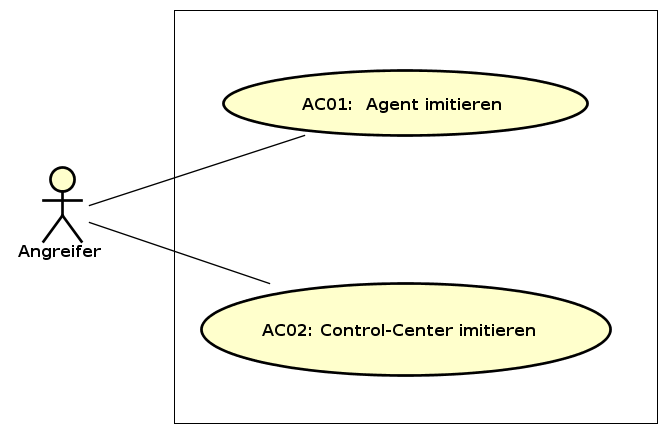
\includegraphics[width=0.75\textwidth]{files/AbuseCases_small}
\end{center}

\xxx[caption!]

\subsection*{AC01: Agent imitieren}
\label{auc:01}

Szenario: Ein Angreifer gibt sich als Agent aus und meldet sich bei CC an. Damit ist es dem Angreifer möglich, das System mit verfälschten Daten zu füttern und dem Systemadmistrator so gezielt falsche Informationen zu vermitteln. Im schlimmsten Fall trifft der Systemadministrator falsche Entscheidungen.

\subsection*{AC02: Control-Center imitieren}
\label{auc:02}

Szenario: Ein Angreifer gibt sich als falsches Control-Center aus und meldet sich beim Agent. Der Angreifer kann Aufträge für Software-Updates erteilen und so direkt auf das System Einfluss nehmen.